\chapter{Wprowadzenie}
\label{cha:wprowadzenie}

$$	\frac{dx}{dt} = \alpha x - \beta x y $$
$$	\frac{dy}{dt} = \delta xy - \gamma y $$

gdzie

\begin{eqwhere}[2cm]
	\item[$x$] liczebność populacji ofiary
	\item[$y$] liczebność populacji drapieżnika
	\item[$\frac{dx}{dt}$,$\frac{dy}{dt}$] przyrost populacji w jednostce czasu
	\item[$t$] czas
	\item[$\alpha$,$\beta$,$\delta$,$\gamma$] parametry opisujące interakcje między populacjami i właściwości populacji
\end{eqwhere}

\noindent Modele ofiar drapieżników są jednymi z najważniejszych elementów składających się na bio- i ekosystemy. Gatunki konkursują, ewoluują, rozprzestrzeniają się dla bolączki poszukiwania pożywienia i możliwości przedłużenia linii garunku. Konkurencja może przyjmować różne formy: drapieżnik-ofiara,wirus-system immulonogiczny, pasożyt-nosiciel, surowiec-konsument, itd. 

\noindent W 1926 słynny Włoski matematyk Vito Volterra zaproponował prosty model opisujący interakcje między ofiarą i drapieżnikiem. Bazuje na kilku założeniach dotyczących środowiska, w którym koegzystują populacje ofiar i drapieżników, to jest:

\begin{itemize}
	\item Ofiara ma zawsze wystarczająco dużo pożywienia.
	
	\item Zaopatrzenie w pożywienie drapieżników zależy wyłącznie od wielkości populacji ofiar.
	
	\item Tempo wzrostu populacji jest proporcjonalne do jej wielkości.
	
	\item Środowisko nie podlega zmianom na korzyść którejkolwiek z populacji, a ewolucja genetyczne jest niekonswekwentna.
	
	\item Drapieżniki mają ograniczony apetyt.
\end{itemize}

\noindent Równania Lotki-Volterry, to para równań różniczkowych I rzędu, nieliniowych.

\noindent Analiza równań mówi nam, że zmiana ilościowa populacji ofiar jest równa jej tempu wzrostu minus  tempo z jaką populacja drapieżników eliminuje ofiary ze środkowiska. Z drugiego zaś biegunu, tempo wzrostu populacji drapieżników jest równoważne tempu wzrostu zasilanym przez dostępność pożywienia minus tempo ubytku populacji na skutek śmierci naturalnej.

\noindent Portret fazowy modelu Lotki-Voleterry daje interesujące rezultaty.

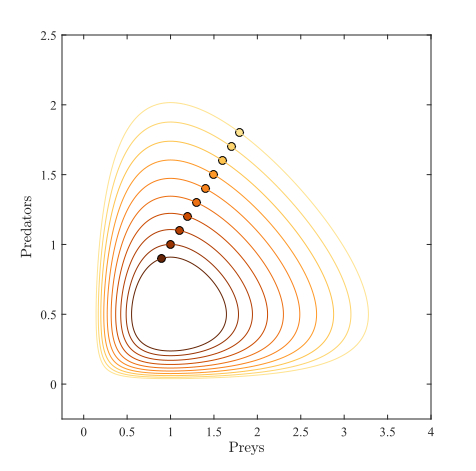
\includegraphics{img/symu}

\noindent Powyższy diagram pokazuje fluktuacje w ilości populacji ofiar i drapieżników. Koła zaznaczona na brzegach zamkniętych powierzchni pokazują warunki początkowe (dla stałych parametrów), gdzie ilości na osiach są rzędu $10^3$. W tym przypadku punktem stałym (populacje obu gatunków są ustalone i nie podlegają zmianom w czasie) jest punkt $(1;0.5)$. 

\noindent W modelu wyraźnie widać, że okres dobrego rozwoju drapiezników przypada gdy populacja ofiar jest duża. Jednakże, poprzez nadmierny rozrost i stopniowe malenie pokładów pożywienia, populacja drapieżników maleje. Wówczas, ofiary nie są na przysłowiowym „celowniku” i mają warunki do rozwoju. Koło się zatoczyło i cykl powtarza się.

\noindent Dla podanego systemu istnieją dwa ekwilibria. Jedno, punkt $(0;0)$, jest równoznaczne wymarciu obu populacji. Taki stan rzeczy będzie się miał  niezależnie od upływającego czasu. Podobnie, drugie ekwilibrium, z obiema populacjami o dodatnich wartościach, jest zależne od początkowych parametrow określających właściwości populacji ofiar i drapieznika.

\noindent Interesujące z biologicznego punktu widzenia jest stabilność układu dla drugiego ekwilibrium. 

\begin{equation}
\lambda_1=i\sqrt{\alpha\gamma} \quad \lambda_2=-i\sqrt{\alpha\gamma}
\end{equation}

\noindent Linearyzacja modelu wokół interesującego punktu: wartości własne jakobianu dla modelu przy drugim ekwilibrium są czysto urojone. Ten krytyczny punkt jest bifurkacją Hopfa – przy niewielkiej zmianie stabilność systemu zmienia się i pojawiają się rozwiązania okresowe. Warto podkreślić, że I metoda Lapunowa nie rozstrzyga o stabilności punktu równowagi, jeżeli system zlinearyzowany jest jedynie stabilny. \cite{Mit}

\noindent Punkt ustalony jest eliptyczny i na podstawie teorii Kolmongorova-Arnolda-Mosera (KAM), która daje odpowiedź na zachowanie w pobliżu punktów eliptycznych, populacje odchylone od punktu ustalonego będą podlegały oscylacjom z częstością $ \omega=\sqrt{\alpha\gamma} $.

\vspace{1cm}
\begin{figure}[ht]
	\centering
	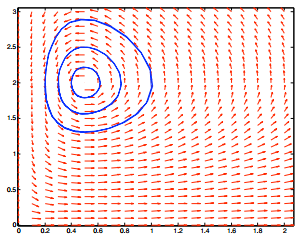
\includegraphics[width=0.6\textwidth]{img/phase}
	\caption{Portret fazowy przedstawionego modelu. Widać oscylujące wokół ekwilbrium rozwiązania i nieograniczony wzrost jednej populacji przy wymarciu drugiej}
\end{figure}













